\chapter{Análisis}


\section{Metodología de desarrollo}

Las metodologías de desarrollo de software surgieron hace décadas como consecuencia de la acumulación de proyectos fallidos o de mala calidad, en los que los resultados no satisfacían al usuario. Esto era debido a que todo el desarrollo seguía el enfoque de los programadores del proyecto, los cuáles no tenían en la mayoría de las ocasiones la misma visión que el usuario para el desarrollo del proyecto.

Hoy en día la elección de una metodología de desarrollo de software es fundamental para el desarrollo de un proyecto de calidad. El uso de una metodología, sin importar de que tipo sea, nos asegura que nuestro proyecto se adecuará a las peticiones del usuario y será un buen producto final.

La implantación de estas metodologías en la mayoría de los proyectos actuales ha aumentado el porcentaje de proyectos que terminan en éxito, y además en los plazos de tiempo.


\subsection{Tipos de metodologías}

Desde que empezó la preocupación por el desarrollo de los proyectos, distintas personas han ido investigando y desarrollando nuevas metodologías. Una posible clasificación de todas estas metodologías puede ser según la época de su creación, teniendo metodologías clásicas y metodologías ágiles.

\subsubsection{Metodología Clásica}

Las metodologías clásicas fueron las primeras metodologías que surgieron como solución al caos que había en la planificación de proyectos. La metodología clásica se caracteriza por una estructura secuencial, es decir, no se vuelve a la etapa anterior una vez se ha completado una etapa de la planificación; además el proceso es rígido y no cambia, es decir, una vez se acuerda como va a ser la planificación, a lo cuál se le dedica grandes cantidades de tiempo, no se modifica nada de la planificación, ni siquiera los requisitos, y por lo tanto la comunicación con el usuario se limita al comienzo del proyecto durante la elaboración la planificación. Aunque viendo su nombre parezca que se trata de una metodología arcaica y en desuso, no es así bajo ningún concepto. Esta metodología se sigue puliendo y mejorando actualmente, aunque uno de sus problemas es su enfoque ``mayorista'', es decir, la metodología está enfocada a los macro-proyectos. Un macro-proyecto es un proyecto con una gran inversión, con un equipo de trabajo de varias decenas de personas, con los roles bien definidos; y con un amplio plazo de tiempo. Aunque un proyecto no encaje con la definición de macro-proyecto, esta metodología se puede adaptar al proyecto en cuestión.

La metodología clásica o metodología ``en cascada'', recibiendo este nombre por ausencia de vuelta a atrás en las etapas, su ciclo de etapas se puede visualizar en la Figura \ref{fig:etapas_clasica}.

\begin{figure}[h]
    \centering
    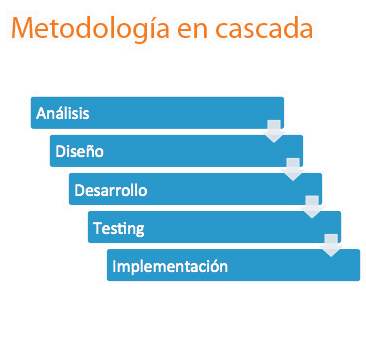
\includegraphics[width=0.6\textwidth]{imagenes/03_Planificacion/meto_clasica.jpg}
    \label{fig:etapas_clasica}
    \begin{center}
        Fuente: \url{https://www.yunbitsoftware.com/blog/2016/05/20/desarrolo-de-software-metodologias-waterfall-agile}
    \end{center}
    \caption{Etapas de la metodología clásica}
\end{figure}


Dado que la metodología clásica sólo consta de un ciclo para realizar las etapas, será imprescindible una buena planificación de alcance, tiempo y coste del proyecto y de cada una de las etapas. Esta planificación inicial es tan importante porque no se obtendrán resultados del proyecto hasta que se encuentre cercano a su cierre.

Entre los problemas de la metodología clásica podemos encontrar los siguientes:

\begin{itemize}
    \item Los proyectos reales difícilmente se adecuan a este modelo de proceso.
    \item Dificultad para expresar por parte del cliente todos los requisitos al principio del proyecto.
    \item Poca comunicación con cliente/usuario, hasta las etapas finales no hay un ejecutable que se pueda evaluar.
\end{itemize}


\subsubsection{Metodología Ágil}

Esta metodología surge como solución a los problemas de la metodología clásica, sobretodo para la planificación de proyectos cortos y cambiantes. La metodología ágil se caracteriza por su flexibilidad, durante el desarrollo del proyecto la planificación sufre continuos cambios debido a la constante comunicación con el usuario; una estructura incremental, con esta metodología no se obtiene un único proyecto final, si no más bien se van generando prototipos que se van analizando y mejorando en un retroalimentación constante, aumentando la colaboración; y un flujo de proceso iterativo, a diferencia de la metodología clásica donde cada etapa una vez finalizada no se vuelve a ella teniendo un flujo en cascada, en esta metodología el flujo de las etapas es más parecido a un círculo convertido en un bucle sin fin. Algo muy importante a tener en cuenta es que a pesar de que los sprints duren poco tiempo esto no permite la falta de documentación, al igual que se hace en la metodología clásica se debe documentar un mínimo a pesar de la brevedad de los sprints. Esta metodología se adapta mejor a los proyectos del ámbito de las TIC, es decir, en el desarrollo de software, donde es fundamental la flexibilidad del proyecto y el carácter incremental de la metodología. Este modo de trabajar no se adecua a proyecto que puedan estar relacionados con sectores alejados de las TIC como puede ser el sector de la construcción, por ejemplo en la construcción de un puente, dado que no se pueden crear prototipos de una construcción ya que no serían seguros, y además son proyectos poco cambiantes en los requisitos del proyecto durante su desarrollo.

El ciclo de etapas de la metodología ágil se puede visualizar en la Figura \ref{fig:etapas_agil}.

\begin{figure}[h]
    \centering
    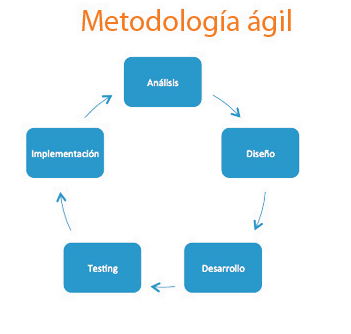
\includegraphics[width=0.6\textwidth]{imagenes/03_Planificacion/meto_agil.jpg}
    \label{fig:etapas_agil}
    \begin{center}
        Fuente: \url{https://www.yunbitsoftware.com/blog/2016/05/20/desarrolo-de-software-metodologias-waterfall-agile}
    \end{center}
    \caption{Etapas de la metodología ágil}
\end{figure}


Dentro de la categoría de metodología ágil podemos encontrar las siguientes metodologías:

\begin{itemize}
    \item Scrum
    \item Programación exterma (XP)
    \item Mobile-D
\end{itemize}

En mi caso me voy a centrar en la metodología Scrum, muy popular hoy en día en la planificación de proyectos TIC. Tal y como se indica en el artículo \cite{RefWorks:RefID:11-cevallos2018metodologias}, Scrum no corresponde a ningún acrónimo, su nombre proviene del deporte rugby, que es una formación requerida para la recuperación rápida del juego ante una infracción menor. Esta metodología se caracteriza por el empleo de un conjunto de reglas y la definición de roles. La existencia de estos roles favorece una colaboración eficaz del equipo de trabajo. 
Los roles que se definen son: El Scrum master, el dueño del producto o Product owner y el equipo de desarrollo o team. El scrum master es la persona que lidera el equipo asegurándose que el equipo cumpla las reglas y procesos de la metodología. El dueño del producto es el representante de los accionistas y clientes que usan el software. El equipo de desarrollo es el grupo de profesionales encargados de convertir la lista de requerimientos o también llamado Product Backlog en funcionalidades del software (Referencia a Articulo metodología).

La característica incremental de las metodologías ágiles se materializa en la metodología Scrum como un elemento llamado Sprint (Figura \ref{fig:sprint_scrum}). Cada sprint consistirá en un recorrido completo de todas las etapas del proyecto, dando como resultado una versión utilizable del producto.

Los elementos de un sprint son los siguientes:

\begin{itemize}
    \item Reunión de planificación del sprint
    \item Daily Scrum ó reunión diaria
    \item Trabajo de desarrollo
    \item Revisión
    \item Retrospectiva del sprint
\end{itemize}

Durante la reunión de planificación del sprint se seleccionan que tareas se van a desarrollar en ese sprint. Las tareas son extraídas del Product Backlog, que no es más que una lista de tareas ordenas por prioridad. Esta lista será actualizada y modificada durante el desarrollo del proyecto.

\begin{figure}[h]
    \centering
    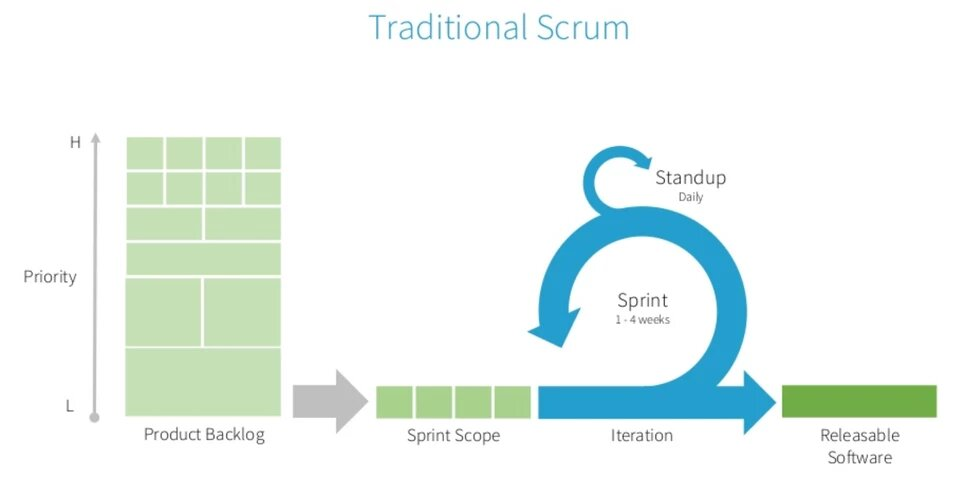
\includegraphics[width=0.8\textwidth]{imagenes/03_Planificacion/sprint_scrum.jpg}
    \begin{center}
        Fuente: \url{https://openwebinars.net/blog/que-es-un-sprint-scrum}
    \end{center}
    \caption{Sprint de la metodología Scrum}
    \label{fig:sprint_scrum}
\end{figure}


\subsection{Comparativa de las metodologías}





\section{Aplicación de Scrum al proyecto}

Tomando como partida la metodología Scrum original, se ha realizado una adaptación a mi proyecto. La primera adaptación es la asignación de roles, donde una misma persona realiza los tres roles a la vez, dado que el equipo de desarrollo del proyecto lo forma una única persona; y como añadido el papel de usuario lo realizará el tutor del proyecto. Otra consecuencia, derivada de la formación del equipo por una única persona, es que no van a realizar reuniones diarias dado que no hay que realizar una supervisión del trabajo del equipo en conjunto. Aunque no se realicen reuniones diarias se ha optado por realizar autorreflexiones semanalmente para llevar un control del avance durante el sprint. Los sprints tendrán una duración inicial de 4 semanas. Además de las propias autorreflexiones, se realizarán reuniones con el tutor cada dos semanas, es decir, inicialmente estas reuniones se producirán a mitad de cada sprint y al final del mismo, aunque el contacto con el tutor es constante durante todo el sprint.

Además de aplicar la metodología Scrum, he optado por aplicar la metodología DevOps. Esta metodología busca la transparencia entre el equipo que desarrolla el software y el equipo que se encarga del despliegue del mismo.



\section{Historias de usuario}

Dado que hemos elegido una metodología SCRUM las características y funcionalidades del sistema no van a estar definidas en función de una lista de requisitos, tal y como se hace en la metodologías tradicionales, indicando los requisitos funcionales, no funcionales y de información; sino que se van a definir por historias de usuario.

Las historias de usuario definen estos requisitos de una forma informal y desde el punto de vista de un rol. La historia de usuario estará formada por una serie de frases, pero las cantidad de frases será escasa, sin generalizar mucho en la funcionalidad descrita en la historia de usuario.

Las frases de las historias de usuario sigue el siguiente patrón: Como \textbf{<rol>}, quiero \textbf{<evento>} para \textbf{<funcionalidad>}.

Además de la frase que describe la funcionalidad, una historia de usuario consta de una frase que indica cuando se considera completada la historia de usuario y de las tareas a realizar.

Una vez definida la estructura de las historias de usuario procedemos a describir cada una de ellas.


\subsection{Tarjetas de historias de usuario}


\begin{table}[h]
\centering
\resizebox{\textwidth}{!}{%
\begin{tabular}{|
>{\columncolor[HTML]{C0C0C0}}c |l|}
\hline
\textbf{Identificación} & HU.1 - Deducción de la edad y el genero                                                                                                     \\ \hline
\textbf{Descripción}    & \begin{tabular}[c]{@{}l@{}}Como usuario quiero que se deduzca mi edad \\ y genero para personalizar las respuesta del chatbot.\end{tabular} \\ \hline
\textbf{Aceptación} &
  \begin{tabular}[c]{@{}l@{}}El sistema debe deducir la edad y el genero en \\ base a una pequeña conversación con el usuario \\ ó en caso de no poder deducir esta información \\ deberá preguntar explícitamente al usuario.\end{tabular} \\ \hline
\textbf{Tareas} &
  \begin{tabular}[c]{@{}l@{}}• Añadir módulo de deducción al sistema antes \\    de comenzar la conversación temática.\\  • Comprobar que se ha deducida la información \\    antes de comenzar la conversación temática.\\  • Realizar la pregunta de la información \\    explícitamente si se detecta que no se conoce.\end{tabular} \\ \hline
\end{tabular}%
}
\caption{Historia de Usuario - HU.1}
\label{tab:HU1}
\end{table}


\begin{table}[H]
\centering
\resizebox{\textwidth}{!}{%
\begin{tabular}{|
>{\columncolor[HTML]{C0C0C0}}c |l|}
\hline
\textbf{Identificación} & HU.2 - Interfaz sencilla \\ \hline
\textbf{Descripción} & \begin{tabular}[c]{@{}l@{}}Como usuario quiero que la interfaz sea sencilla\\ para facilitar su uso por cualquier persona.\end{tabular} \\ \hline
\textbf{Aceptación}  & \begin{tabular}[c]{@{}l@{}}La interfaz debe tener una estructura de conversación\\ sencilla, de pregunta-respuesta.\end{tabular}        \\ \hline
\textbf{Tareas}      & \begin{tabular}[c]{@{}l@{}}• Integrar en el sistema una interfaz de conversación\\ estructuralmente sencilla.\end{tabular}              \\ \hline
\end{tabular}%
}
\caption{Historia de Usuario - HU.2}
\label{tab:HU2}
\end{table}


\begin{table}[H]
\centering
\resizebox{\textwidth}{!}{%
\begin{tabular}{|
>{\columncolor[HTML]{C0C0C0}}c |l|}
\hline
\textbf{Identificación} & HU.3 - Interfaz armónica                             \\ \hline
\textbf{Descripción} &
  \begin{tabular}[c]{@{}l@{}}Como usuario quiero que la interfaz siga la armonía\\ del sistema para el uso de la misma sea agradable\\ para el usuario.\end{tabular} \\ \hline
\textbf{Aceptación} &
  \begin{tabular}[c]{@{}l@{}}La interfaz debe mantener la apariencia que tiene el\\ resto del sistema.\end{tabular} \\ \hline
\textbf{Tareas}         & • Integrar la apariencia del sistema en la interfaz. \\ \hline
\end{tabular}%
}
\caption{Historia de Usuario - HU.3}
\label{tab:HU3}
\end{table}


\begin{table}[H]
\centering
\resizebox{\textwidth}{!}{%
\begin{tabular}{|
>{\columncolor[HTML]{C0C0C0}}c |l|}
\hline
\textbf{Identificación} & HU.4 - Interfaz responsive          \\ \hline
\textbf{Descripción} &
  \begin{tabular}[c]{@{}l@{}}Como usuario quiero que la interfaz se adapte al\\ dispositivo que esté utilizando en cada momento\\ para aumentar el volumen de gente que podrá\\ utilizar el sistema.\end{tabular} \\ \hline
\textbf{Aceptación} &
  \begin{tabular}[c]{@{}l@{}}La interfaz debe adaptarse al tamaño de la página\\ del dispositivo que esté utilizando el usuario.\end{tabular} \\ \hline
\textbf{Tareas}         & • Elaborar una interfaz responsive. \\ \hline
\end{tabular}%
}
\caption{Historia de Usuario - HU.4}
\label{tab:HU4}
\end{table}


\begin{table}[H]
\centering
\resizebox{\textwidth}{!}{%
\begin{tabular}{|
>{\columncolor[HTML]{C0C0C0}}c |l|}
\hline
\textbf{Identificación} &
  HU.5 - Conversación a tiempo real \\ \hline
\textbf{Descripción} &
  \begin{tabular}[c]{@{}l@{}}Como usuario quiero que la respuesta del sistema\\ se genere en un corto periodo de tiempo para\\ que su uso se haga más natural y entretenido.\end{tabular} \\ \hline
\textbf{Aceptación} &
  \begin{tabular}[c]{@{}l@{}}El sistema debe generar las respuesta y proporcio-\\ narselas al usuario en un corto periodo de tiempo\\ como podría ser como máximo 5 segundos.\end{tabular} \\ \hline
\textbf{Tareas} &
  \begin{tabular}[c]{@{}l@{}}• Implementar un sistema eficiente en cuanto al\\ tiempo necesario para lageneración de las res-\\ puestas.\end{tabular} \\ \hline
\end{tabular}%
}
\caption{Historia de Usuario - HU.5}
\label{tab:HU5}
\end{table}


\begin{table}[H]
\centering
\resizebox{\textwidth}{!}{%
\begin{tabular}{|
>{\columncolor[HTML]{C0C0C0}}c |l|}
\hline
\textbf{Identificación} & HU.6 - Conversación coherente \\ \hline
\textbf{Descripción} &
  \begin{tabular}[c]{@{}l@{}}Como usuario quiero que las respuestas del sistema\\ tenga una coherencia con el resto de la conversación \\ realizada con anterioridad a la pregunta de la\\ respuesta esperada para que su uso sea más agradable\\ e interesante para el usuario.\end{tabular} \\ \hline
\textbf{Aceptación} &
  \begin{tabular}[c]{@{}l@{}}Las respuestas del sistema deben tener cierta coherencia\\ con la conversación realizada hasta ese momento, ha-\\ ciendo uso de la información proporcionada por el\\ usuario para generar la respuesta.\end{tabular} \\ \hline
\textbf{Tareas} &
  \begin{tabular}[c]{@{}l@{}}• Implementar un mecanismo que incluya la información\\ proporcionada por el usuario en la generación de las \\ respuestas.\\  • Implementar un mecanismo que genere distintas repues-\\ tas según la información deducida del usuario por el mó-\\ dulo de deducción.\end{tabular} \\ \hline
\end{tabular}%
}
\caption{Historia de Usuario - HU.6}
\label{tab:HU6}
\end{table}


\begin{table}[H]
\centering
\resizebox{\textwidth}{!}{%
\begin{tabular}{|
>{\columncolor[HTML]{C0C0C0}}c |l|}
\hline
\textbf{Identificación} &
  HU.7 - Conversación temática \\ \hline
\textbf{Descripción} &
  \begin{tabular}[c]{@{}l@{}}Como administrador del sistema quiero que el sistema \\ genere respuesta relacionada con la IA para fomentar\\ su aprendizaje y uso por parte del usuario.\end{tabular} \\ \hline
\textbf{Aceptación} &
  \begin{tabular}[c]{@{}l@{}}El sistema debe orientar la respuesta a cierta pregunta \\ hacia el ámbito de la IA, sin importar que pregunta se \\ haya realizado.\end{tabular} \\ \hline
\textbf{Tareas} &
  \begin{tabular}[c]{@{}l@{}}• Implementar un sistema que sea capaz de orientar las\\ respuestas al campo de la IA.\\  • Implementar un sistema que genere respuestas sobre\\ la IA personalizándola al usuario en base a la informa-\\ ción proporcionada por el mismo.\end{tabular} \\ \hline
\end{tabular}%
}
\caption{Historia de Usuario - HU.7}
\label{tab:HU7}
\end{table}


\newpage

\subsection{Listado de las historias de usuario}

Una vez se han definido todas las historias de usuario debemos clasificar las historias de usuario por algún criterio para decidir cuáles tienen un mayor impacto en el sistema y decidir cuáles abarcar en un primer momento a la hora de ser implementadas las funcionalidades descritas en las historias. Este criterio será el nivel de prioridad. El nivel de prioridad toma valores desde 1 hasta 3.


\begin{table}[h]
\centering
\resizebox{\textwidth}{!}{%
\begin{tabular}{|c|l|c|}
\hline
\rowcolor[HTML]{C0C0C0} 
\textbf{Identificador} &
  \multicolumn{1}{c|}{\cellcolor[HTML]{C0C0C0}\textbf{Descripción}} &
  \textbf{Prioridad} \\ \hline
HU.1 &
  \begin{tabular}[c]{@{}l@{}}Como usuario quiero que se deduzca mi edad\\ y genero para personalizar las respuesta del chatbot.\end{tabular} &
  3 \\ \hline
HU.2 &
  \begin{tabular}[c]{@{}l@{}}Como usuario quiero que la interfaz sea sencilla\\ para facilitar su uso por cualquier persona.\end{tabular} &
  2 \\ \hline
HU.3 &
  \begin{tabular}[c]{@{}l@{}}Como usuario quiero que la interfaz siga la armonía\\ del sistema para el uso de la misma sea agradable\\ para el usuario.\end{tabular} &
  1 \\ \hline
HU.4 &
  \begin{tabular}[c]{@{}l@{}}Como usuario quiero que la interfaz se adapte al\\ dispositivo que esté utilizando en cada momento\\ para aumentar el volumen de gente que podrá\\ utilizar el sistema.\end{tabular} &
  2 \\ \hline
HU.5 &
  \begin{tabular}[c]{@{}l@{}}Como usuario quiero que la respuesta del sistema\\ se genere en un corto periodo de tiempo para\\ que su uso se haga más natural y entretenido.\end{tabular} &
  3 \\ \hline
HU.6 &
  \begin{tabular}[c]{@{}l@{}}Como usuario quiero que las respuestas del sistema\\ tenga una coherencia con el resto de la conversación\\ realizada con anterioridad a la pregunta de la\\ respuesta esperada para que su uso sea más agradable\\ e interesante para el usuario.\end{tabular} &
  3 \\ \hline
HU.7 &
  \begin{tabular}[c]{@{}l@{}}Como administrador del sistema quiero que el sistema\\ genere respuesta relacionada con la IA para fomentar\\ su aprendizaje y uso por parte del usuario.\end{tabular} &
  2 \\ \hline
\end{tabular}%
}
\caption{Listado de historias de usuario junto con su prioridad}
\label{tab:listado_HU}
\end{table}


\section{Requisitos adicionales}

\begin{itemize}
    \item \textbf{Robustez:} El chatbot deberá responder siempre sin importar que mensaje envíe el usuario.
    \item \textbf{Documentación:} Se incluirá información a modo de manual de usuario para facilitar la utilización del sistema y el ajuste de sus parámetros.
    \item \textbf{Extensibilidad:} El chatbot debe estar preparado para ser fácilmente escalado y tener la suficiente potencia para cumplir sus requisitos.
    \item \textbf{Costo:} El costo final de implementación del sistema debe ser bajo, para ello el sistema debe usar la menor cantidad de recursos sin perder la potencia necesaria.
    \item \textbf{Seguridad:} Se deben mantener privados todos los datos proporcionados por el usuario durante su conversación con el chatbot.
\end{itemize}



\section{Análisis de riesgos}



